\section{Benchmarking \irace hyperparameters}
Given that \irace has not being applied to tackle \nasbench, we study its performance with different setups for a fair comparison with the other \nasbench techniques. We note that when dealing with known benchmarks, ACs can benefit from tailored setups as they can exploit known characteristics of the benchmarks.

% \leslie{}{NOTE: I would suggest to omit the experiments with fixed number of configurations and also the ones that set the configuration budget as number of experiments, as they are not the best performing and it might simplify the analysis.}

We performed 20 repetitions of \irace setting 10 million TPU seconds as total configuration budget and evaluate the performance obtained by the following setup options:

\begin{description}[style=unboxed, leftmargin=0px]
\item[Estimation budget] Budget assigned for the initial estimation of the average execution time of an evaluation. We perform experiments with 2\% and 0.2\% of the total configuration time for budget estimation.
\item[First test] Number of evaluations required to perform the first elimination test in a race. We perform experiments with 2 and 3 evaluations for applying the initial test.
\end{description}

For further details of these setup options we refer to~\cite{LopDubPerStuBir2016irace}. Figure~\ref{fig:irace-setup-performance} gives the ECDFs of the final quality obtained by the different setups of \irace. The best overall performance is obtained by setting the estimation budget to $2\%$ of the total configuration time and allowing 3 evaluations before the first elimination test (mean test regret $0.002837$).
\begin{figure*}
	\centering
	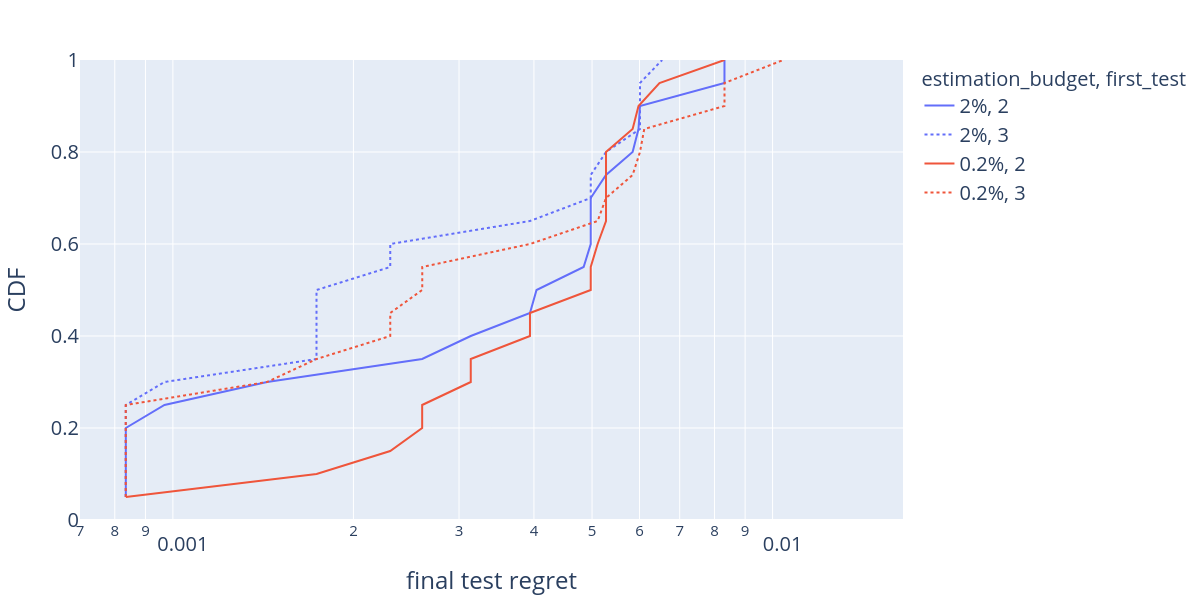
\includegraphics[width=0.75\textwidth]{imgs/irace-setup-ecdf.png}
	\caption{Empirical cumulative distribution function~($x$-axis) of the final regret~($y$-axis) from 20 runs of each \irace setup.}
	\label{fig:irace-setup-performance}
\end{figure*}

\section{High-performing configurations plots}
Here we present parallel categories plots representing the architectures selected by the different NAS techniques. Figure~\ref{fig:pc-fnn} shows the configurations selected when using a fixed number of nodes, while Figure~\ref{fig:pc-vnn} shows those using a variable number of nodes. As in the paper, only NAS hyperpameters related to the node label list are given~(\textit{op$_1$}-\textit{op$_5$}), corresponding to each vertex of the DAG model, i.e. each layer of the selected neural network, for legibility's sake. Furthermore, color scaling (on the same range for all plots) reflects the mean test regret, also depicted as a discretized variable in the left-most column of the plots. Do note that, since topology is defined by the adjacency matrix, no layer order or architecture size should be assumed.

\begin{figure*}
\centering
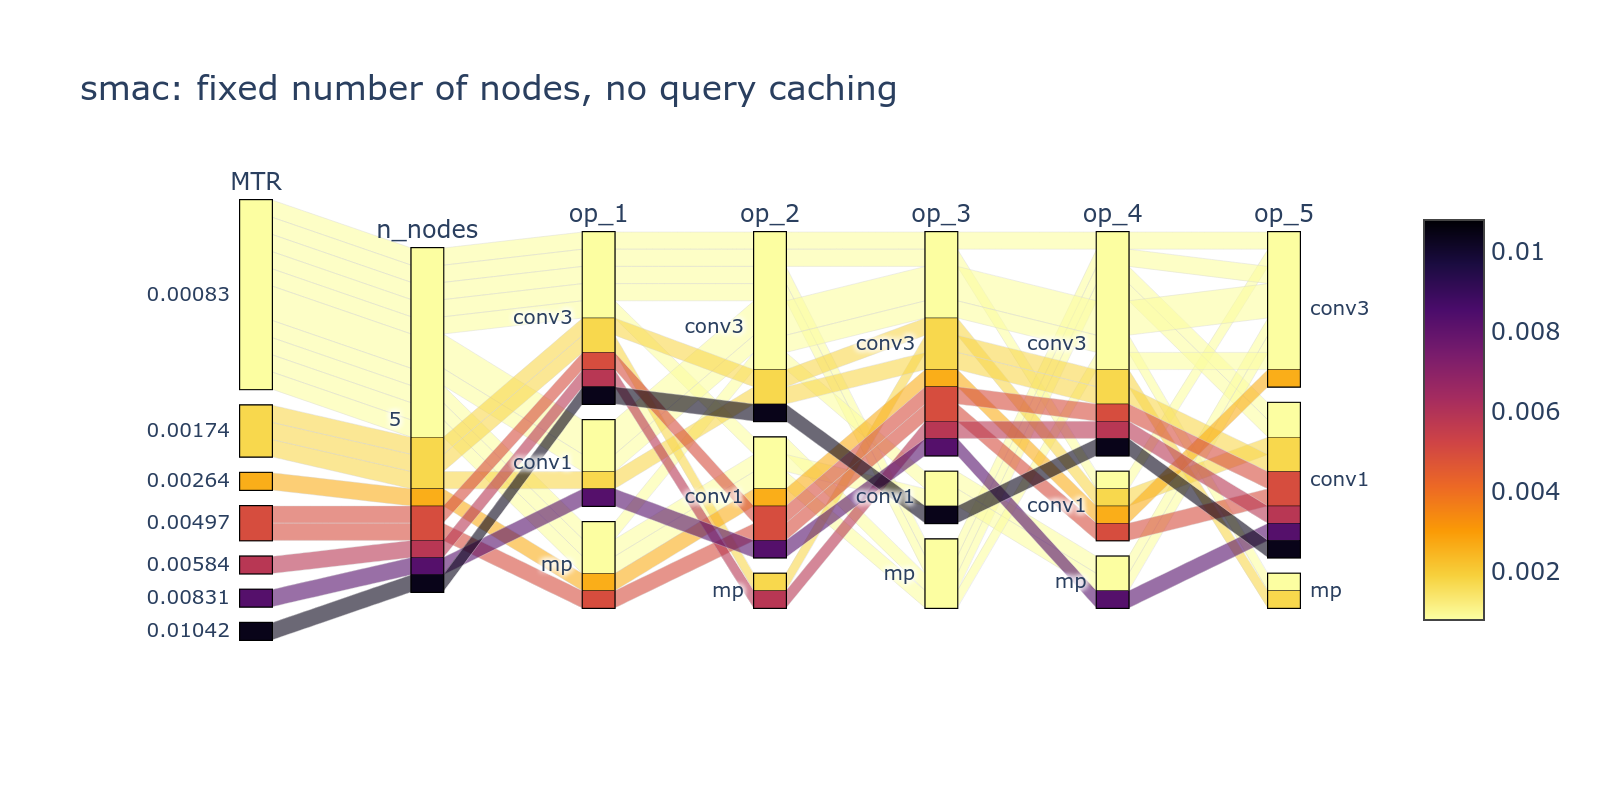
\includegraphics[width=0.47\linewidth, clip=true, trim=140px 150px 40px 150px]{imgs/parcat/smac-fnn-nc.png}
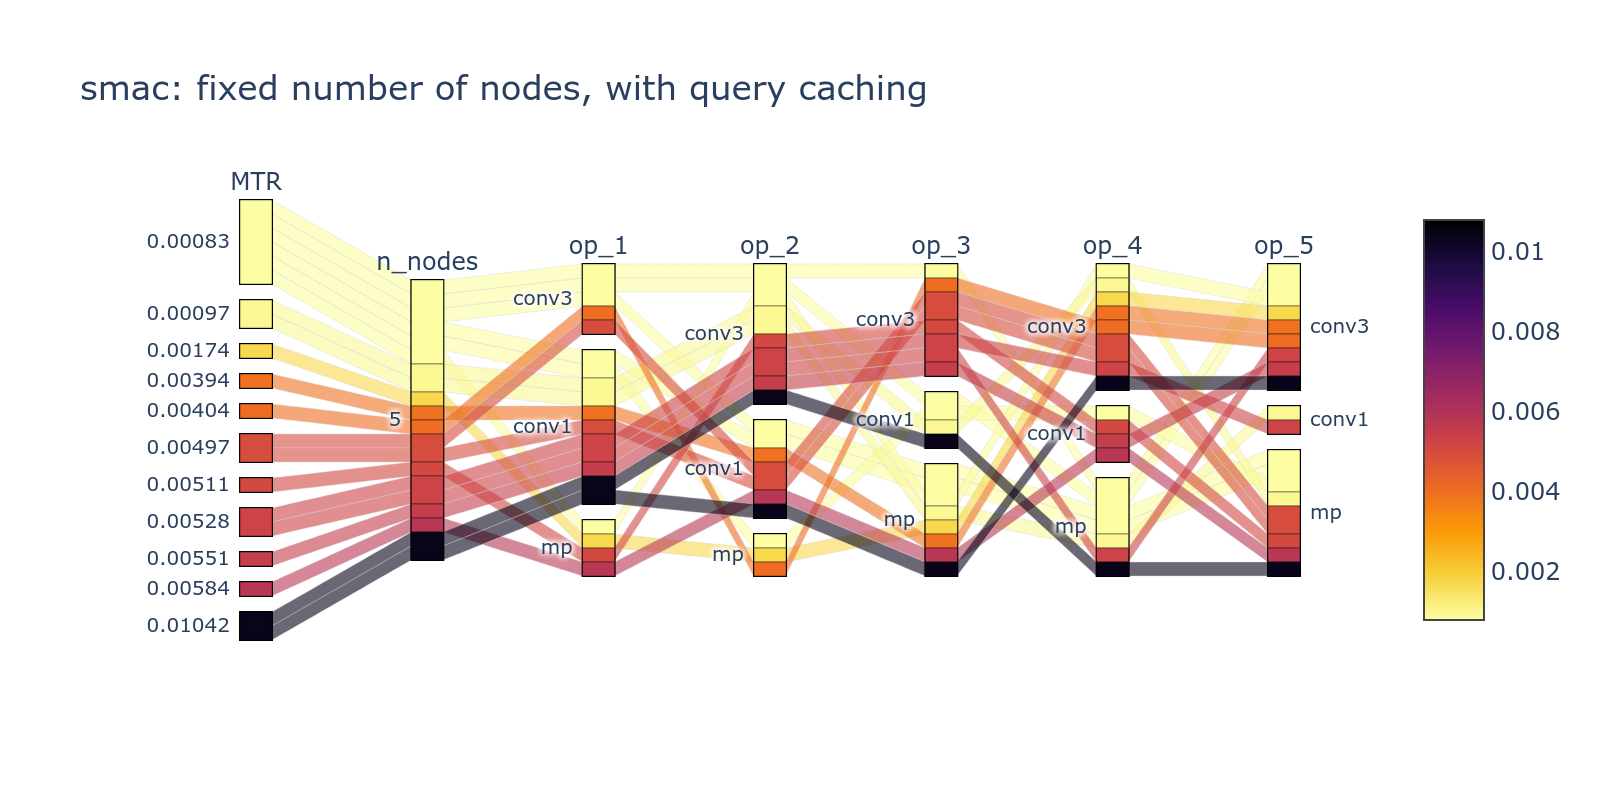
\includegraphics[width=0.47\linewidth, clip=true, trim=140px 150px 40px 150px]{imgs/parcat/smac-fnn.png}
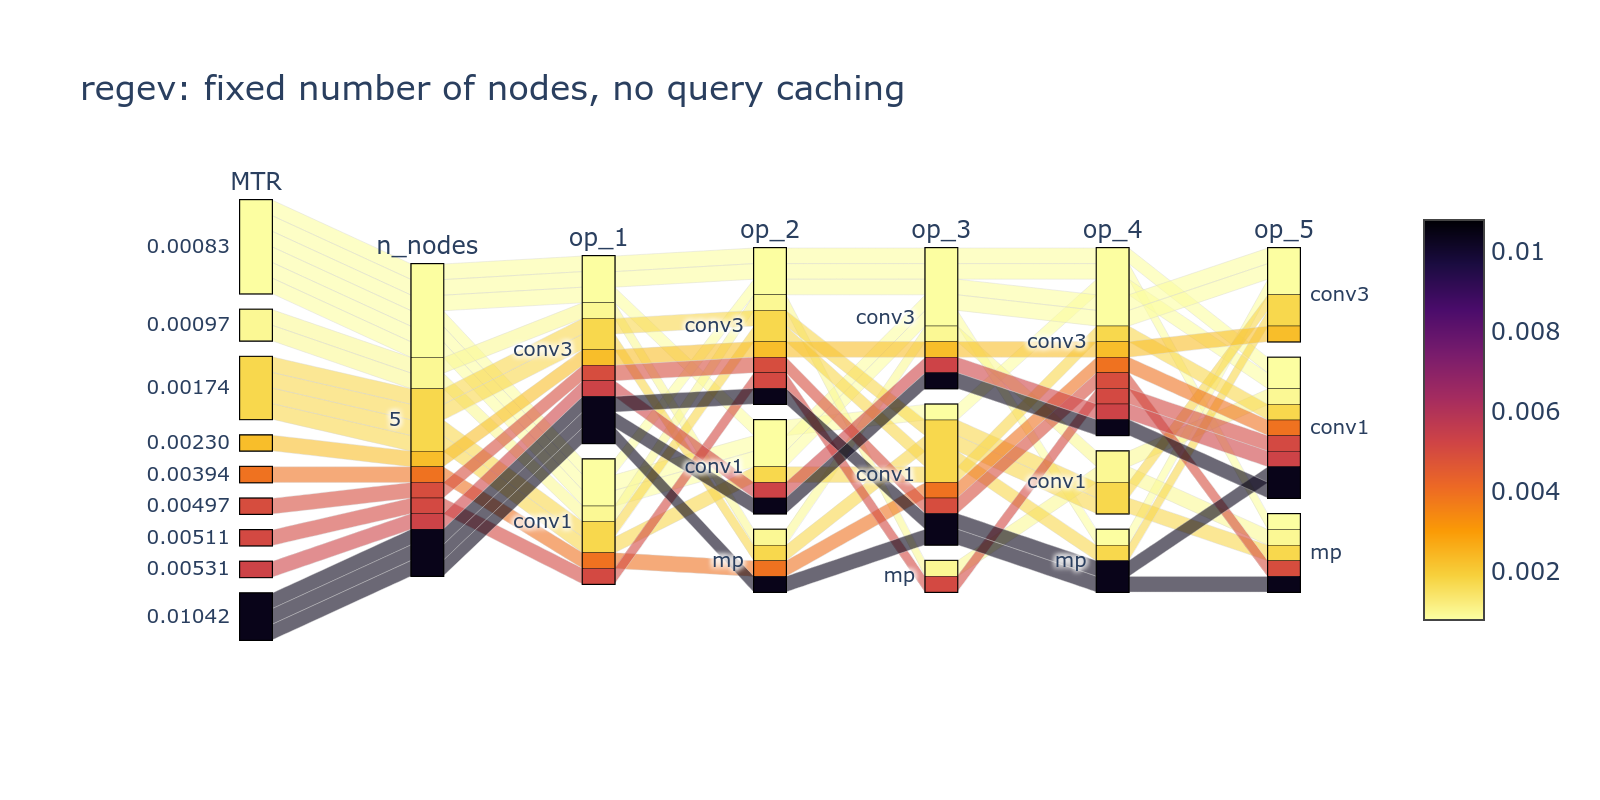
\includegraphics[width=0.47\linewidth, clip=true, trim=140px 150px 40px 150px]{imgs/parcat/re-fnn-nc.png}
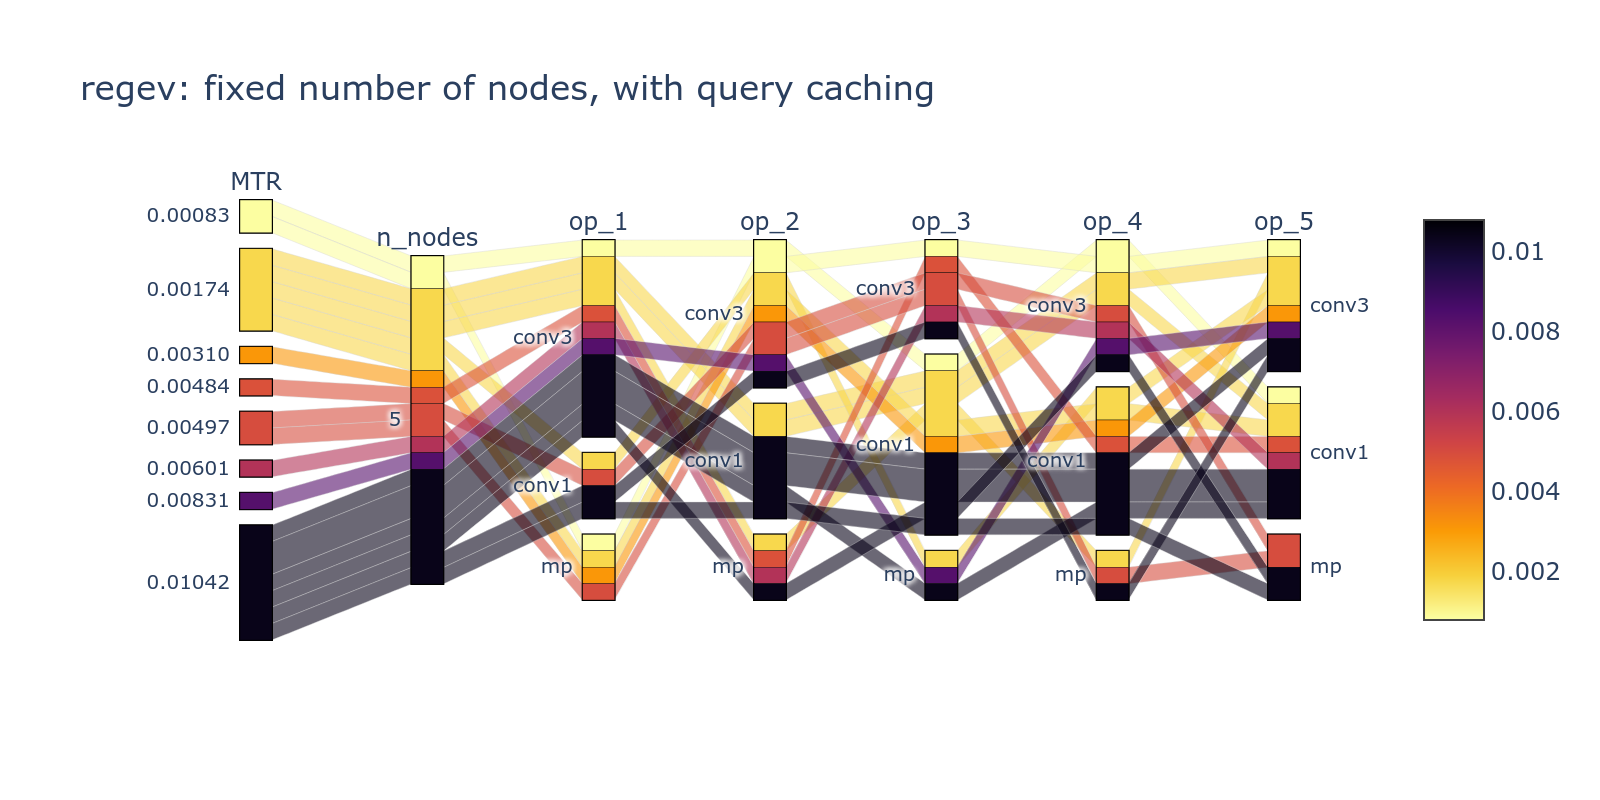
\includegraphics[width=0.47\linewidth, clip=true, trim=140px 150px 40px 150px]{imgs/parcat/re-fnn.png}
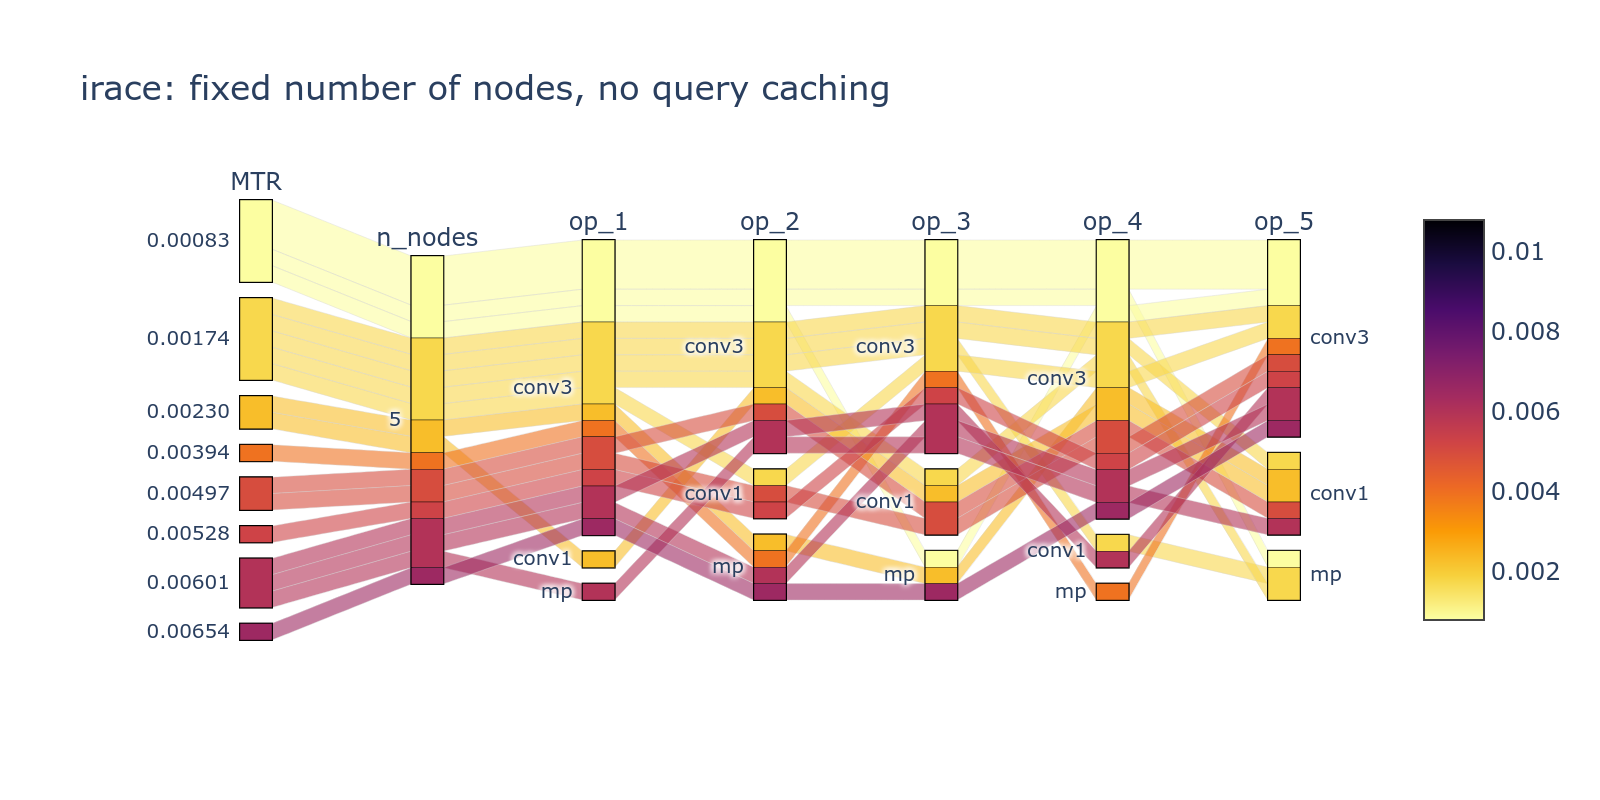
\includegraphics[width=0.47\linewidth, clip=true, trim=140px 150px 40px 150px]{imgs/parcat/irace-fnn-nc.png}
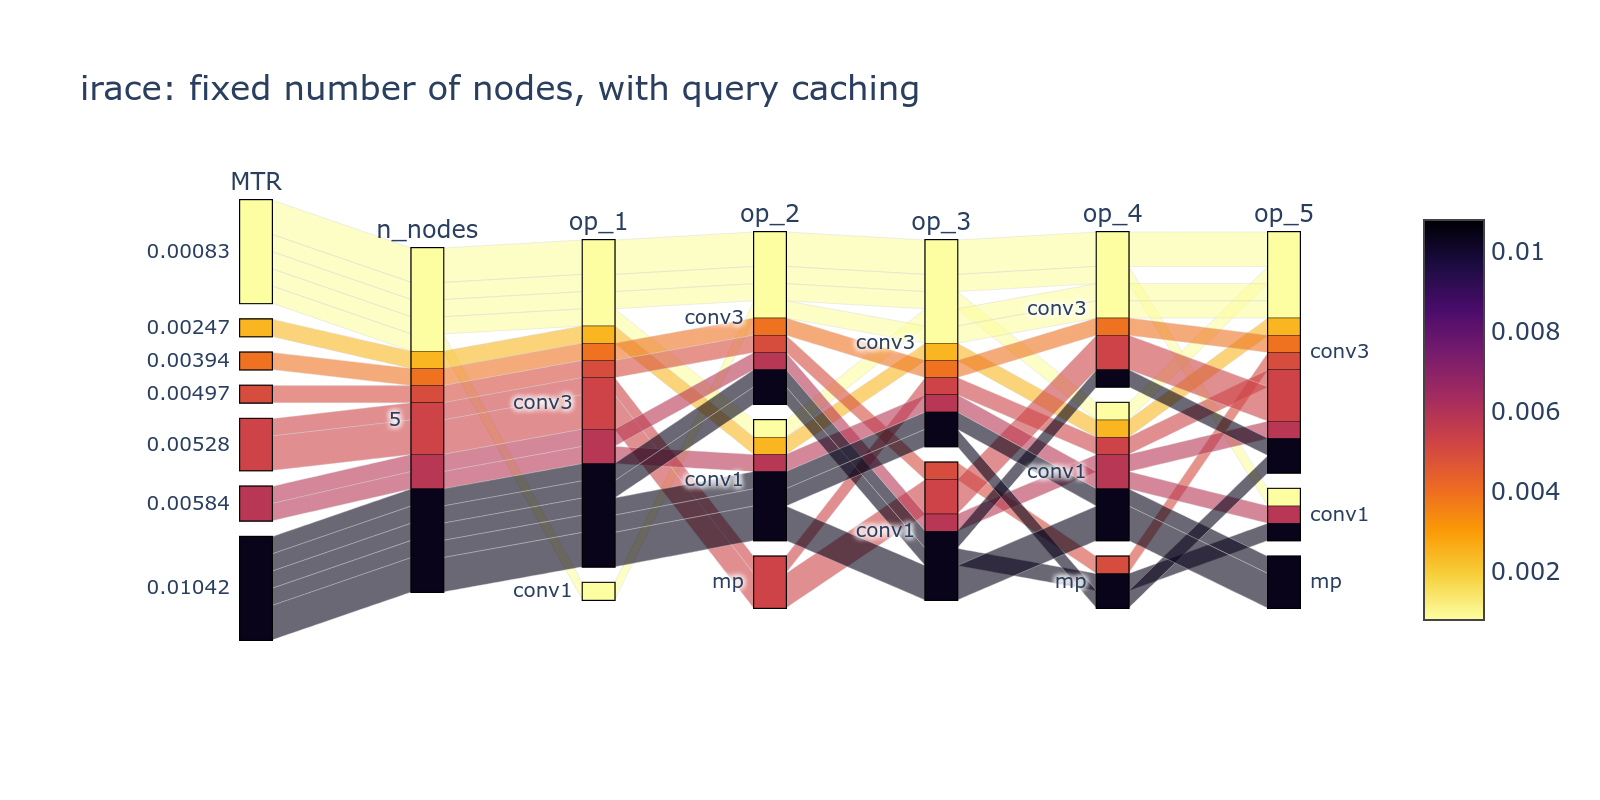
\includegraphics[width=0.47\linewidth, clip=true, trim=140px 150px 40px 150px]{imgs/parcat/irace-fnn.png}
\caption{Parallel categories plots of the 20 architectures selected by SMAC (top), RE (middle), and \irace (bottom) with fixed number of nodes, no caching (left), caching (right).}
\label{fig:pc-fnn}
\end{figure*}


\begin{figure*}
\centering
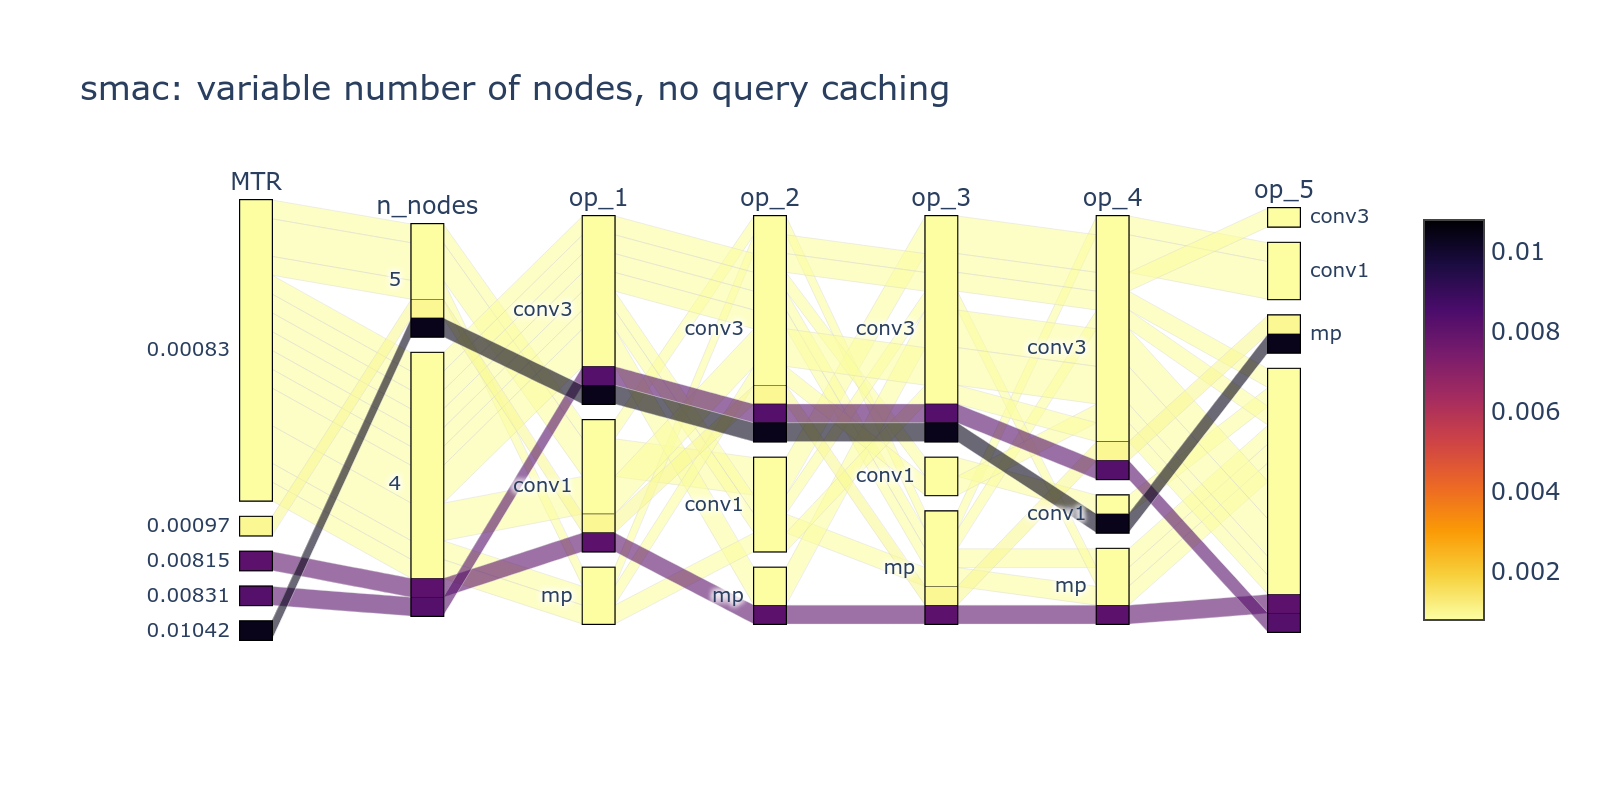
\includegraphics[width=0.47\linewidth, clip=true, trim=140px 150px 40px 150px]{imgs/parcat/smac-vnn-nc.png}
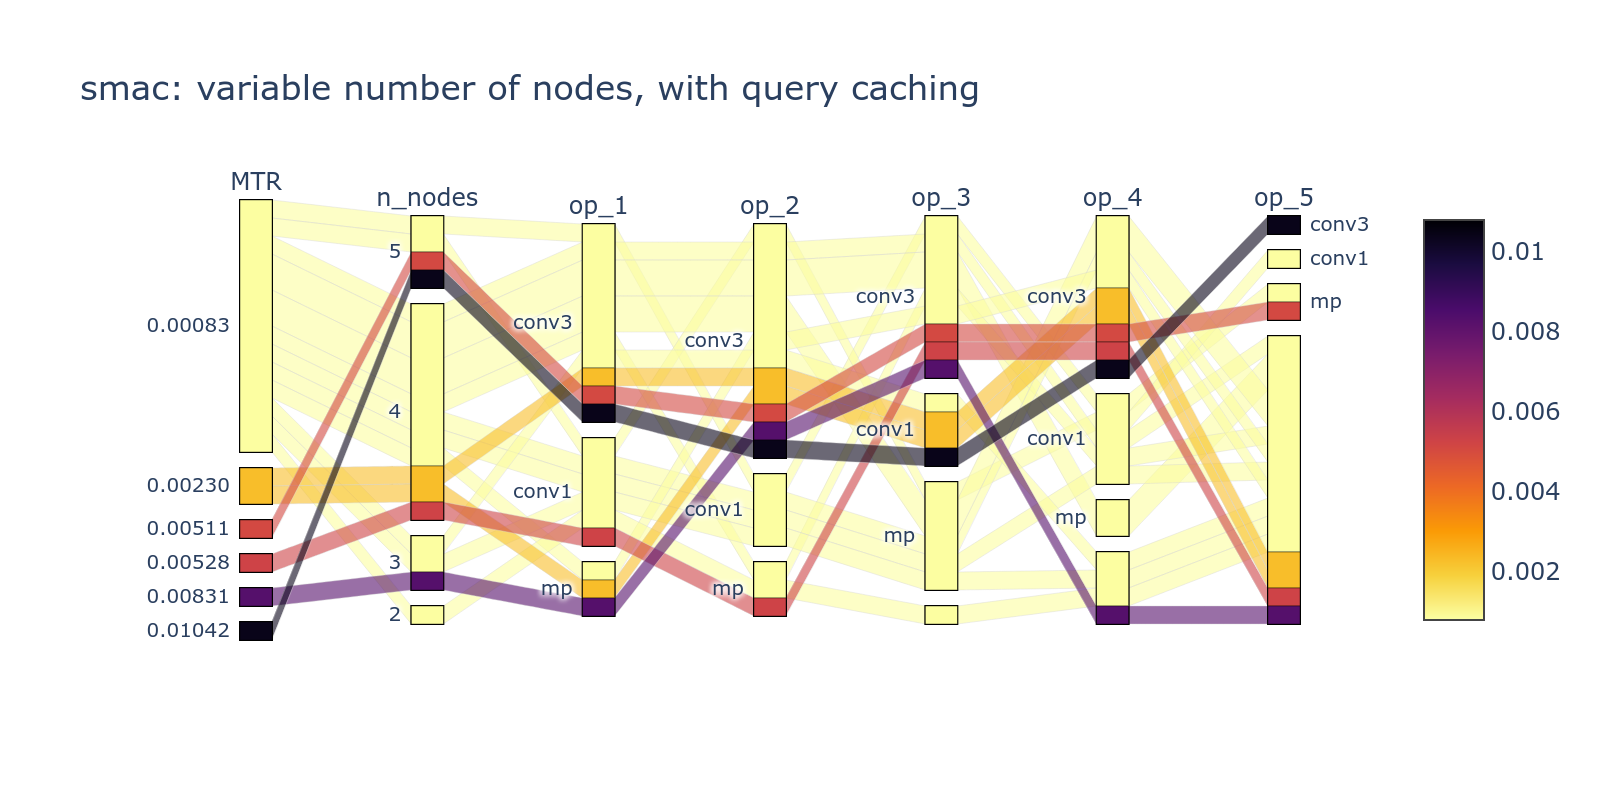
\includegraphics[width=0.47\linewidth, clip=true, trim=140px 150px 40px 150px]{imgs/parcat/smac-vnn.png}
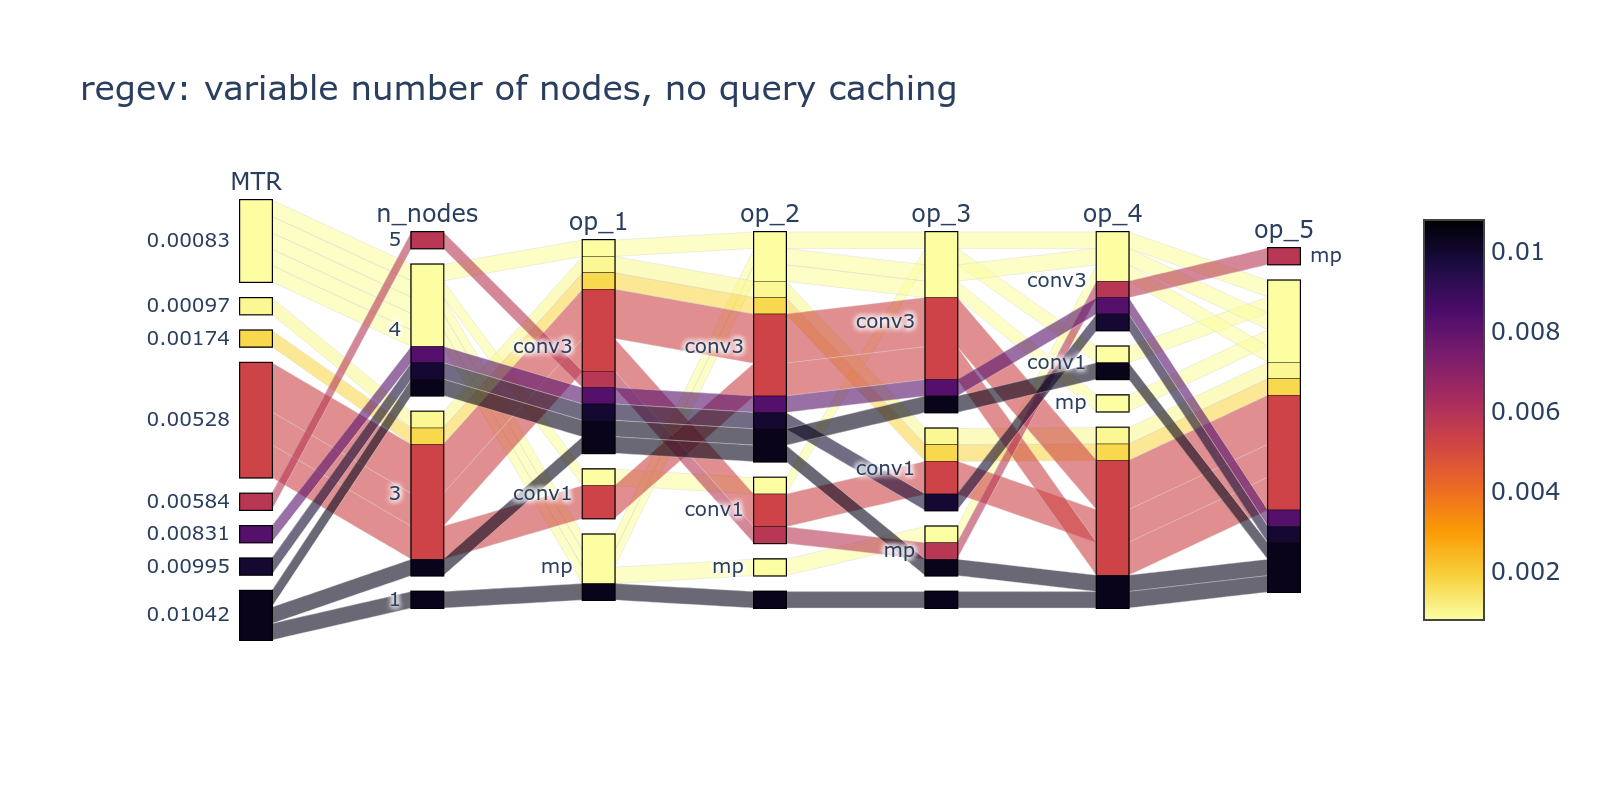
\includegraphics[width=0.47\linewidth, clip=true, trim=140px 150px 40px 150px]{imgs/parcat/re-vnn-nc.png}
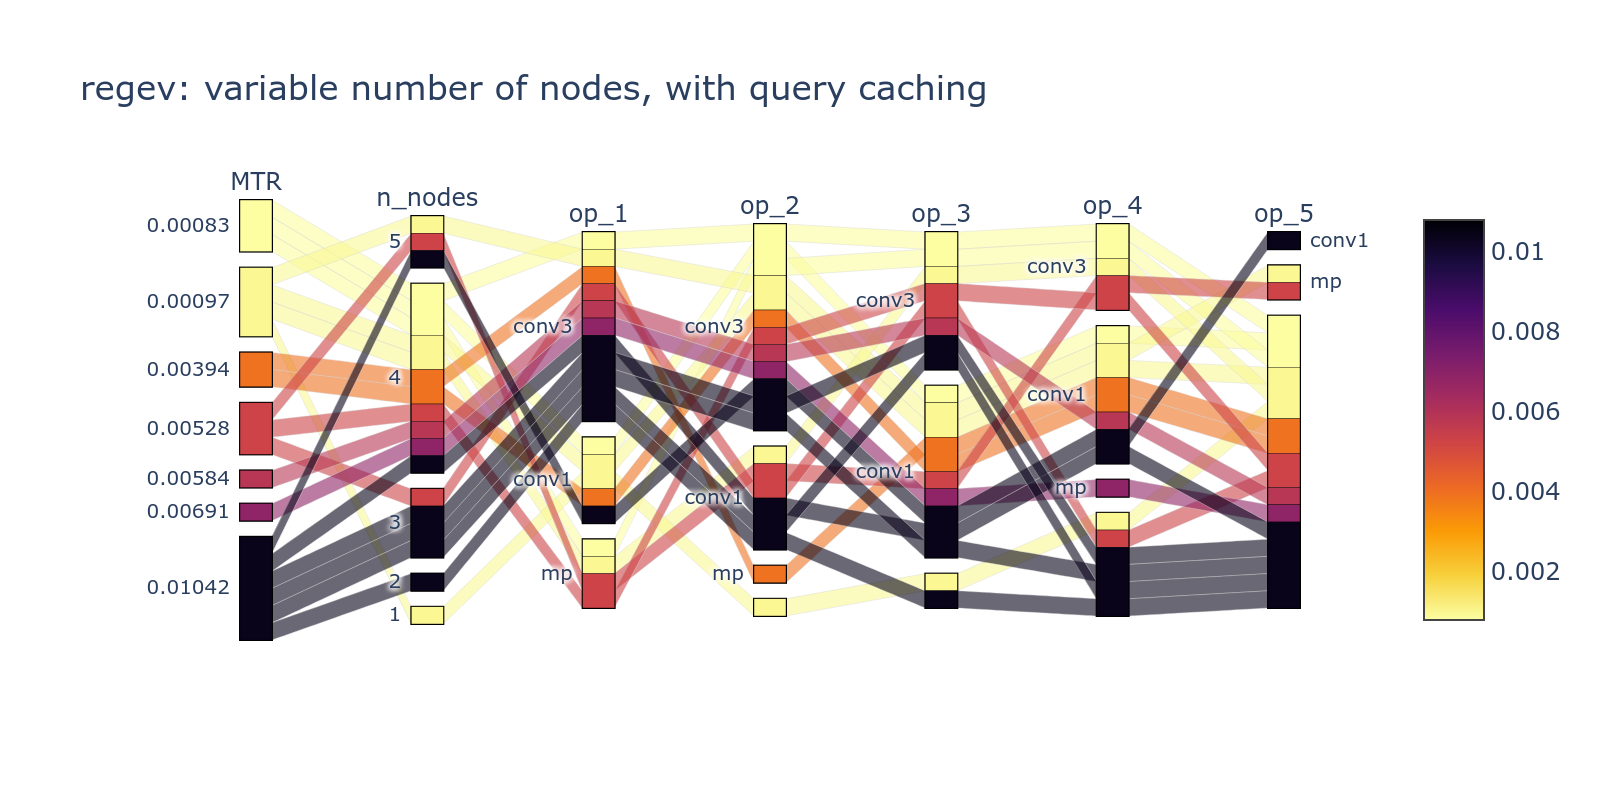
\includegraphics[width=0.47\linewidth, clip=true, trim=140px 150px 40px 150px]{imgs/parcat/re-vnn.png}
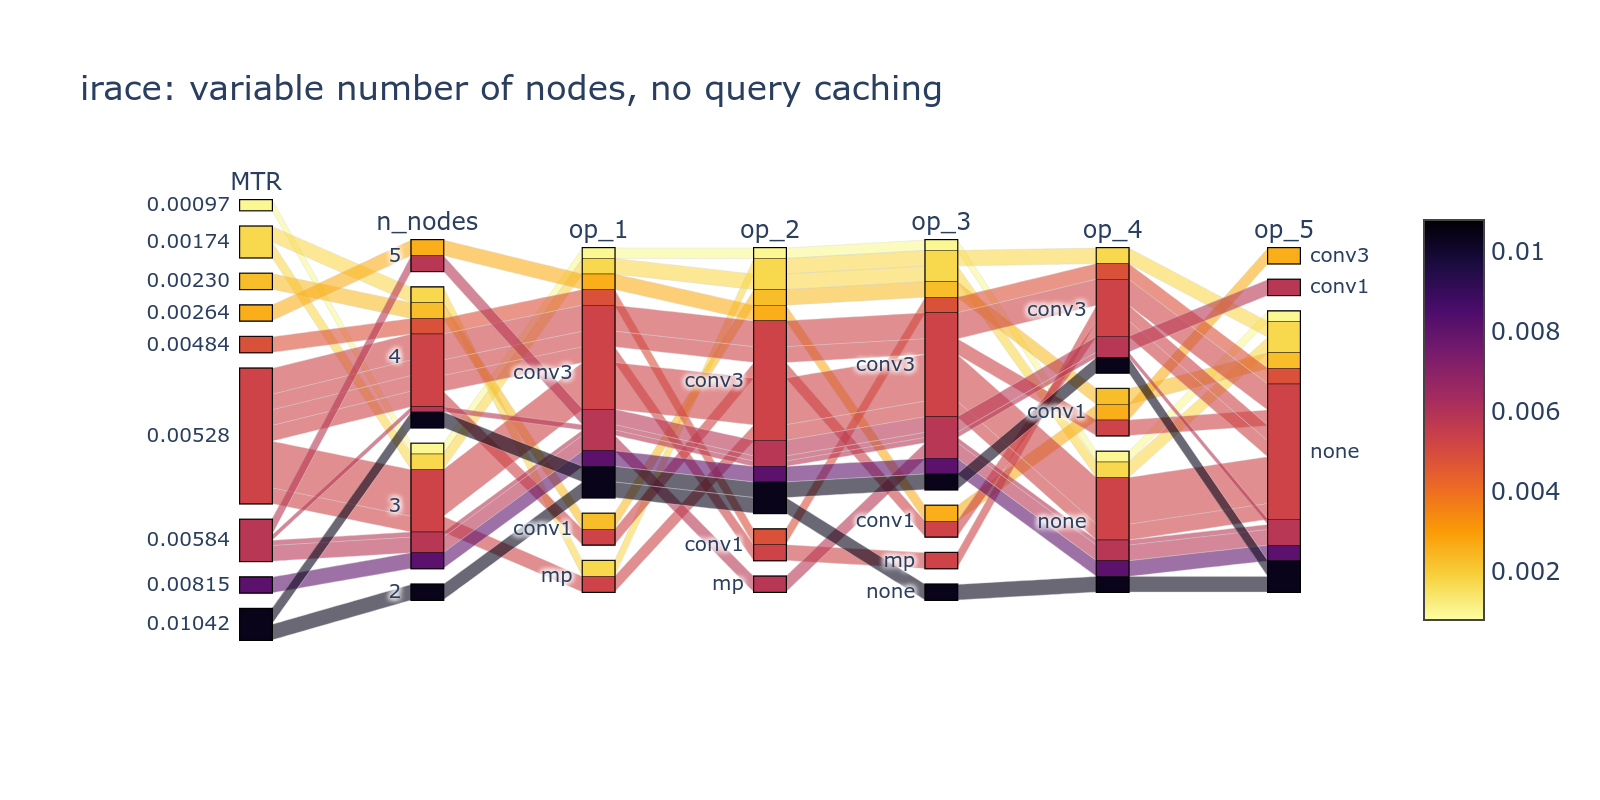
\includegraphics[width=0.47\linewidth, clip=true, trim=140px 150px 40px 150px]{imgs/parcat/irace-vnn-nc.png}
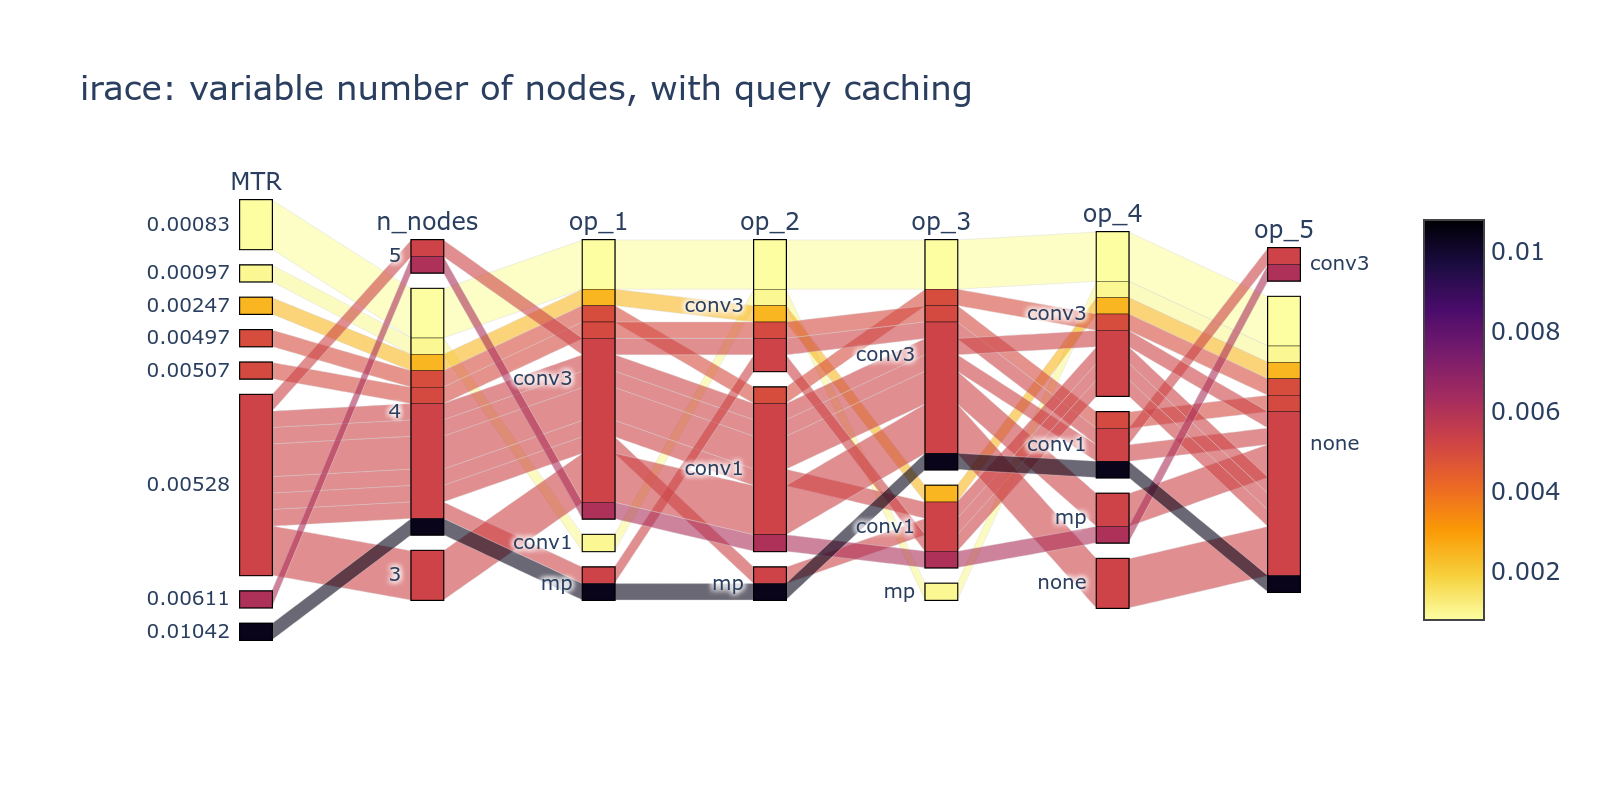
\includegraphics[width=0.47\linewidth, clip=true, trim=140px 150px 40px 150px]{imgs/parcat/irace-vnn.png}
\caption{Parallel categories plots of the 20 architectures selected by SMAC (top) RE (middle) and \irace (bottom) with variable number of nodes, no caching (left), caching (right).}
\label{fig:pc-vnn}
\end{figure*}

\section{Runtime statistics}
Here we give runtime (wallclock) statistics for all three algorithms in their different experimental setups in Figure~\ref{fig:wallclock-times}. Abbreviations for experimental setups are used as in the paper: O for original; VS for variable-sized; C for caching; and CVS for caching and variable-sized. Runtime along the $y$ axis is given in hours:minutes:seconds format.

% \begin{figure*}
% 	\centering

% 	\begin{subfigure}[t]{0.3\textwidth}
% 	\centering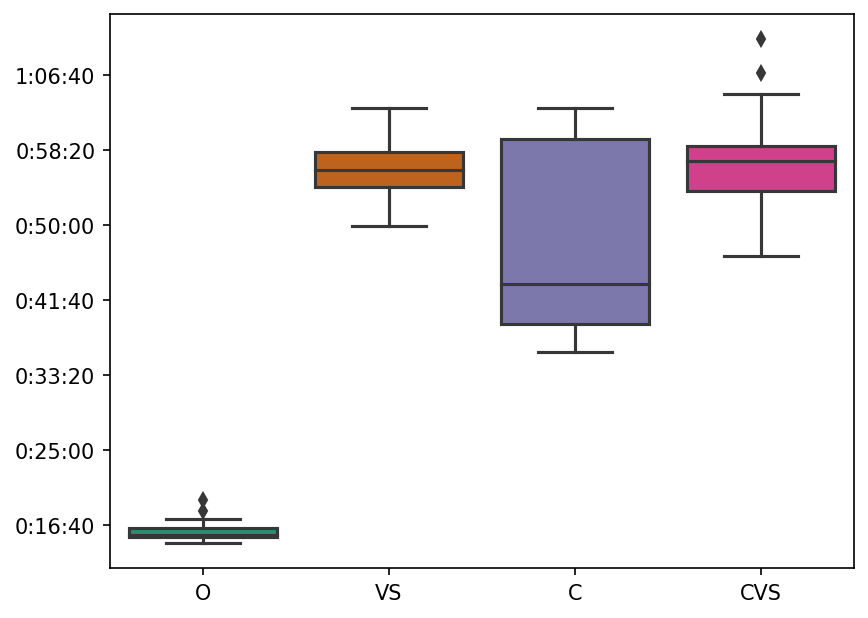
\includegraphics[width=\textwidth]{imgs/irace-times-boxplots.png}
% 	% \caption{\irace}
% 	\end{subfigure}
% 	\begin{subfigure}[t]{0.3\textwidth}
% 	\centering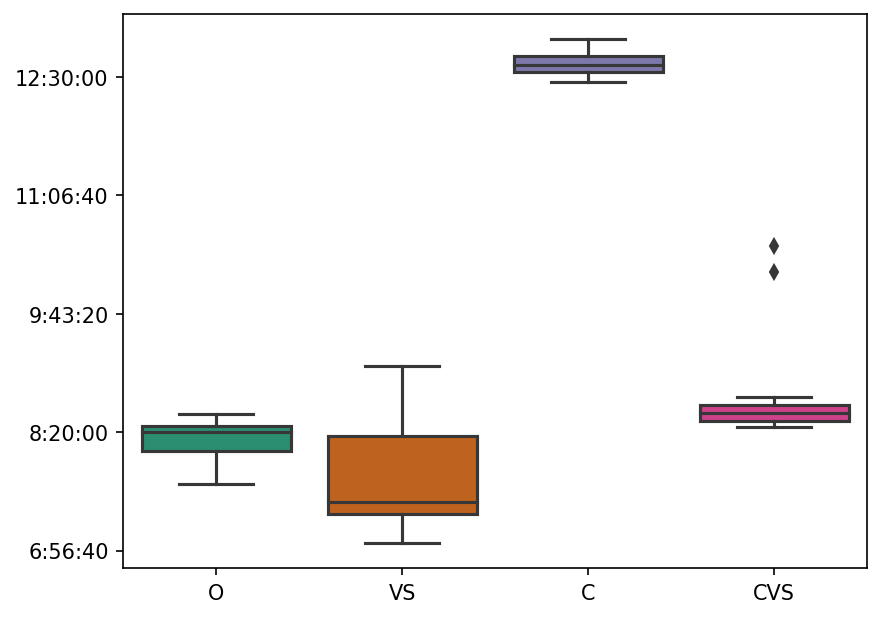
\includegraphics[width=\textwidth]{imgs/smac-times-boxplots.png}
% 	% \caption{SMAC}
% 	\end{subfigure}[t]{0.3\textwidth}
% 	\begin{subfigure}
% 	\centering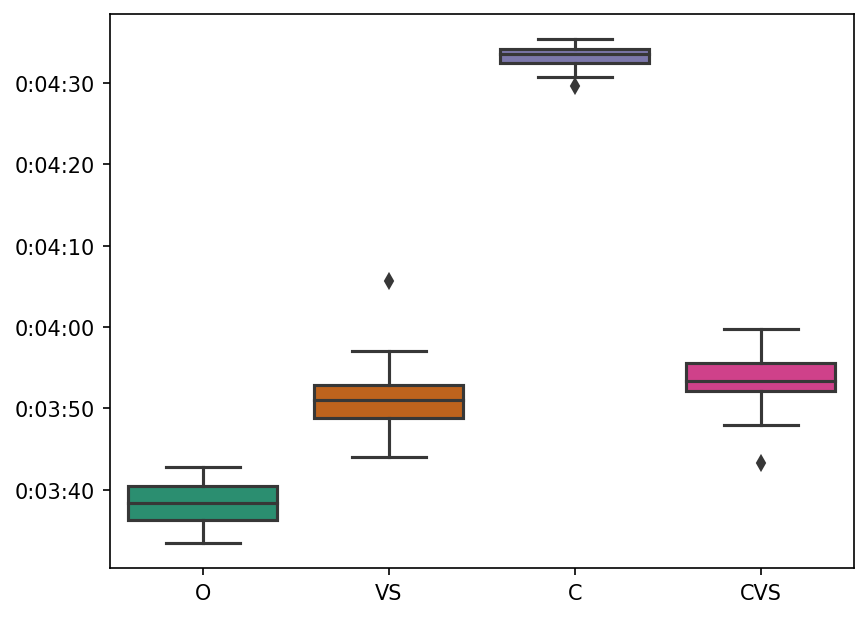
\includegraphics[width=\textwidth]{imgs/regev-times-boxplots.png}
% 	% \caption{RE}
% 	\end{subfigure}

% 	\caption{Boxplots representing wallclock runtimes (over 20 runs) of each algorithm under different experimental setups}
% 	\label{fig:wallclock-times}
% \end{figure*}

\begin{figure*}
\centerline{%
\subfigure[\irace]{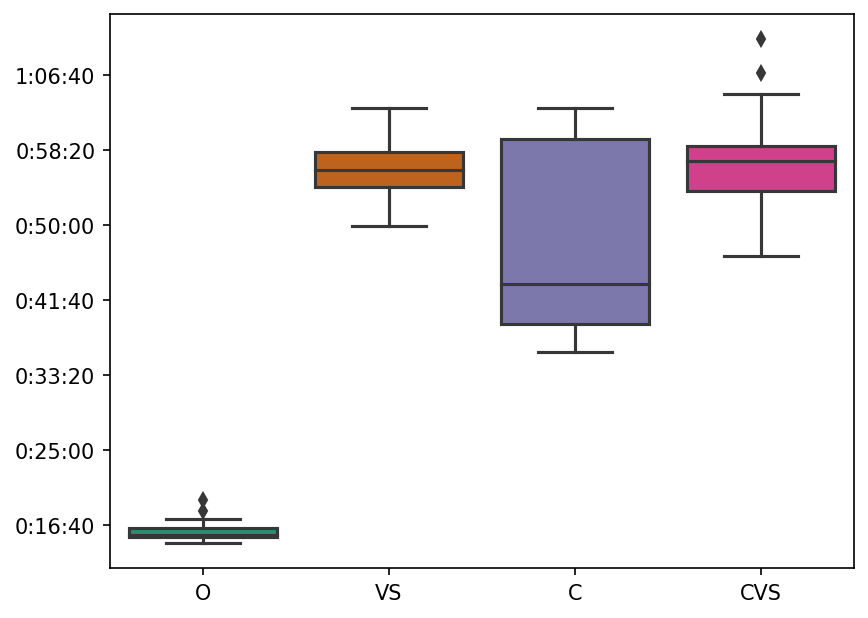
\includegraphics[width=0.3\textwidth]{imgs/irace-times-boxplots.png}}
\hfil
\subfigure[SMAC]{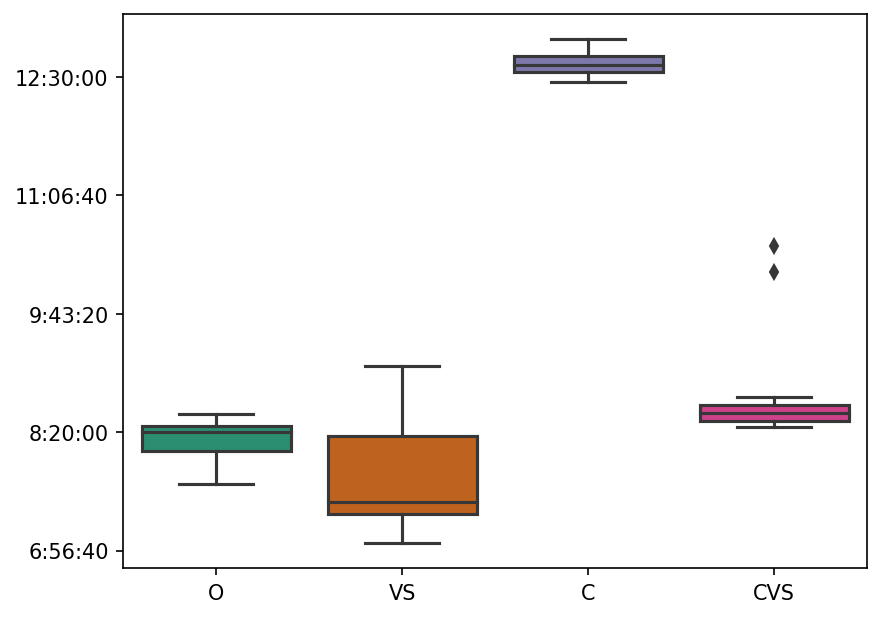
\includegraphics[width=0.3\textwidth]{imgs/smac-times-boxplots.png}}
\hfil
\subfigure[RE]{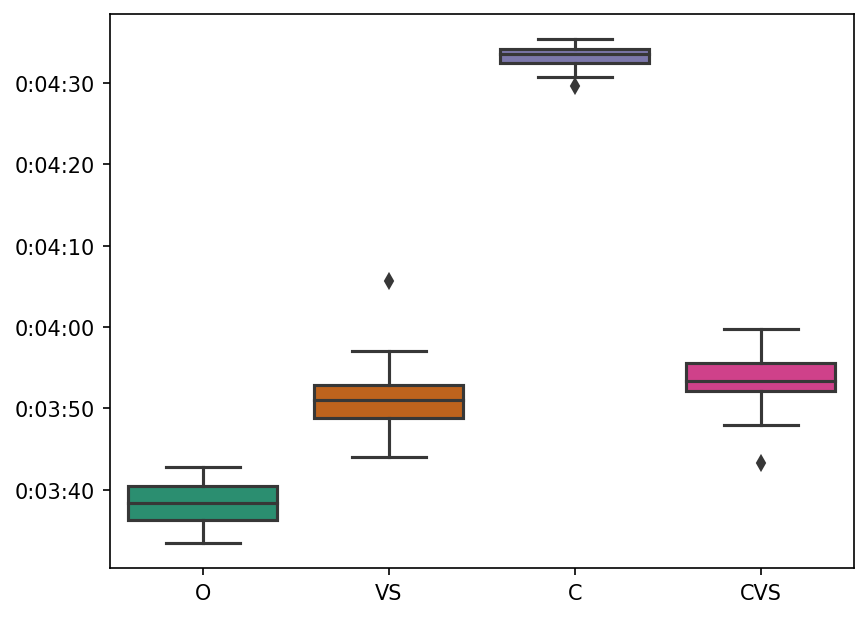
\includegraphics[width=0.3\textwidth]{imgs/regev-times-boxplots.png}}
}
\caption{Boxplots representing wallclock runtimes (over 20 runs) of each algorithm under different experimental setups}
\label{fig:wallclock-times}
\end{figure*}